\documentclass[11pt,a4paper]{article}
\usepackage[utf8]{inputenc}\usepackage[T1]{fontenc}
\usepackage[spanish,es-noshorthands,es-noquoting]{babel}
\usepackage[margin=1.8cm]{geometry}
\usepackage{graphicx,booktabs,xcolor,tcolorbox,enumitem}
\tcbuselibrary{skins,breakable}
\definecolor{azul}{HTML}{24618C}\definecolor{rojo}{HTML}{C0392B}\definecolor{verde}{HTML}{27632A}
\newtcolorbox{aviso}[1]{colback=rojo!6,colframe=rojo,fonttitle=\bfseries,title=#1,breakable,left=3mm,right=3mm,top=2mm,bottom=2mm}
\newtcolorbox{nota}[1]{colback=azul!6,colframe=azul,fonttitle=\bfseries,title=#1,breakable,left=3mm,right=3mm,top=2mm,bottom=2mm}
\newtcolorbox{truco}[1]{colback=verde!6,colframe=verde,fonttitle=\bfseries,title=#1,breakable,left=3mm,right=3mm,top=2mm,bottom=2mm}
\setlength{\parskip}{4pt}\pagestyle{empty}
\begin{document}
\begin{center}
{\LARGE\bfseries Diagramas del sistema}\\[1.5mm]
{\small DaVinci Paddle Boat · Reto EIA 2027 · Marymount}
\end{center}

\begin{nota}{Por qué solo dos diagramas}
El código de cada ejercicio son \textbf{60--99 líneas} con 1--4 \texttt{TODO}: cabe en una
pantalla y se lee, no se dibuja. Diagramarlo enseñaría que el diagrama es lo que se mira y
el código lo que se ignora. Lo que \emph{sí} necesita dibujo es lo que no cabe en la
cabeza: en qué estado está el barco, y la cadena entera del mando al agua.

Los dos salen de \texttt{diagramas/*.mmd} con \texttt{python3 build.py}, que rehace a la
vez las imágenes, este PDF y la nota del Vault. \textbf{Fuente única.}
\end{nota}

\section*{1. Los estados del barco}
Lo más difícil de \emph{Phase 5}, y un concepto de \textbf{seguridad}: mientras el barco no
esté armado, el motor no gira pase lo que pase.

\begin{center}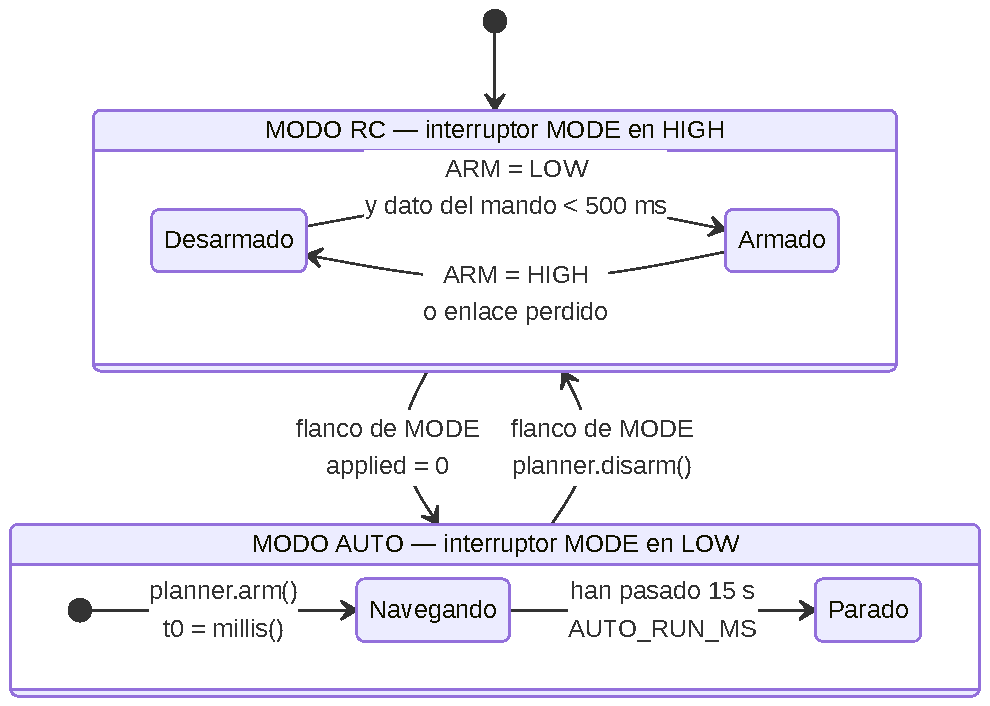
\includegraphics[width=\textwidth]{estados-e5.pdf}\end{center}

Hay \textbf{dos cosas independientes} que se confunden:

\begin{center}\begin{tabular}{@{}lll@{}}\toprule
 & \textbf{Quién lo decide} & \textbf{Qué significa} \\ \midrule
\textbf{Modo} & el interruptor MODE (GPIO 26) & de dónde vienen las órdenes: mando o planificador \\
\textbf{Armado} & el interruptor ARM (GPIO 32) \textbf{y} el failsafe & si se les hace caso, o se manda 0 \\
\bottomrule\end{tabular}\end{center}

Se puede estar en AUTO y desarmado, y en RC y desarmado. \textbf{El modo no arma nada.}

\subsection*{El failsafe tiene dos gatillos}
\texttt{applyFailsafe()} fuerza \texttt{armed = false} si se cumple \textbf{cualquiera}:
\begin{enumerate}[leftmargin=*,itemsep=1pt]
\item El interruptor ARM está abierto (lee HIGH).
\item La orden más reciente tiene más de \texttt{FAILSAFE\_MS} = \textbf{500 ms}.
\end{enumerate}
El segundo es el que salva el barco: si el mando se apaga o se sale de rango, no sigue
navegando con el último \texttt{throttle} recibido.

\begin{truco}{Detalle que se pasa por alto}
En el flanco de cambio de modo, \texttt{applied} se pone a \textbf{0}: la rampa de
aceleración empieza de cero. Sin eso, al saltar a AUTO el barco arrancaría de golpe con la
velocidad que llevaba.
\end{truco}

\begin{center}\begin{tabular}{@{}ll@{}}\toprule
\textbf{LED} & \textbf{Estado} \\ \midrule
Fijo & armado --- el motor puede girar \\
Parpadeo lento (400 ms) & RC, desarmado \\
Parpadeo rápido (150 ms) & AUTO, desarmado o run terminado \\
\bottomrule\end{tabular}\end{center}

\clearpage
\section*{2. Del mando al agua}
Éste es \textbf{el} diagrama del proyecto: el único sitio donde el firmware y todo el
trabajo mecánico aparecen juntos. Azul lo que se programa, rojo lo que se conecta, marrón
lo que se corta y se imprime.

\begin{center}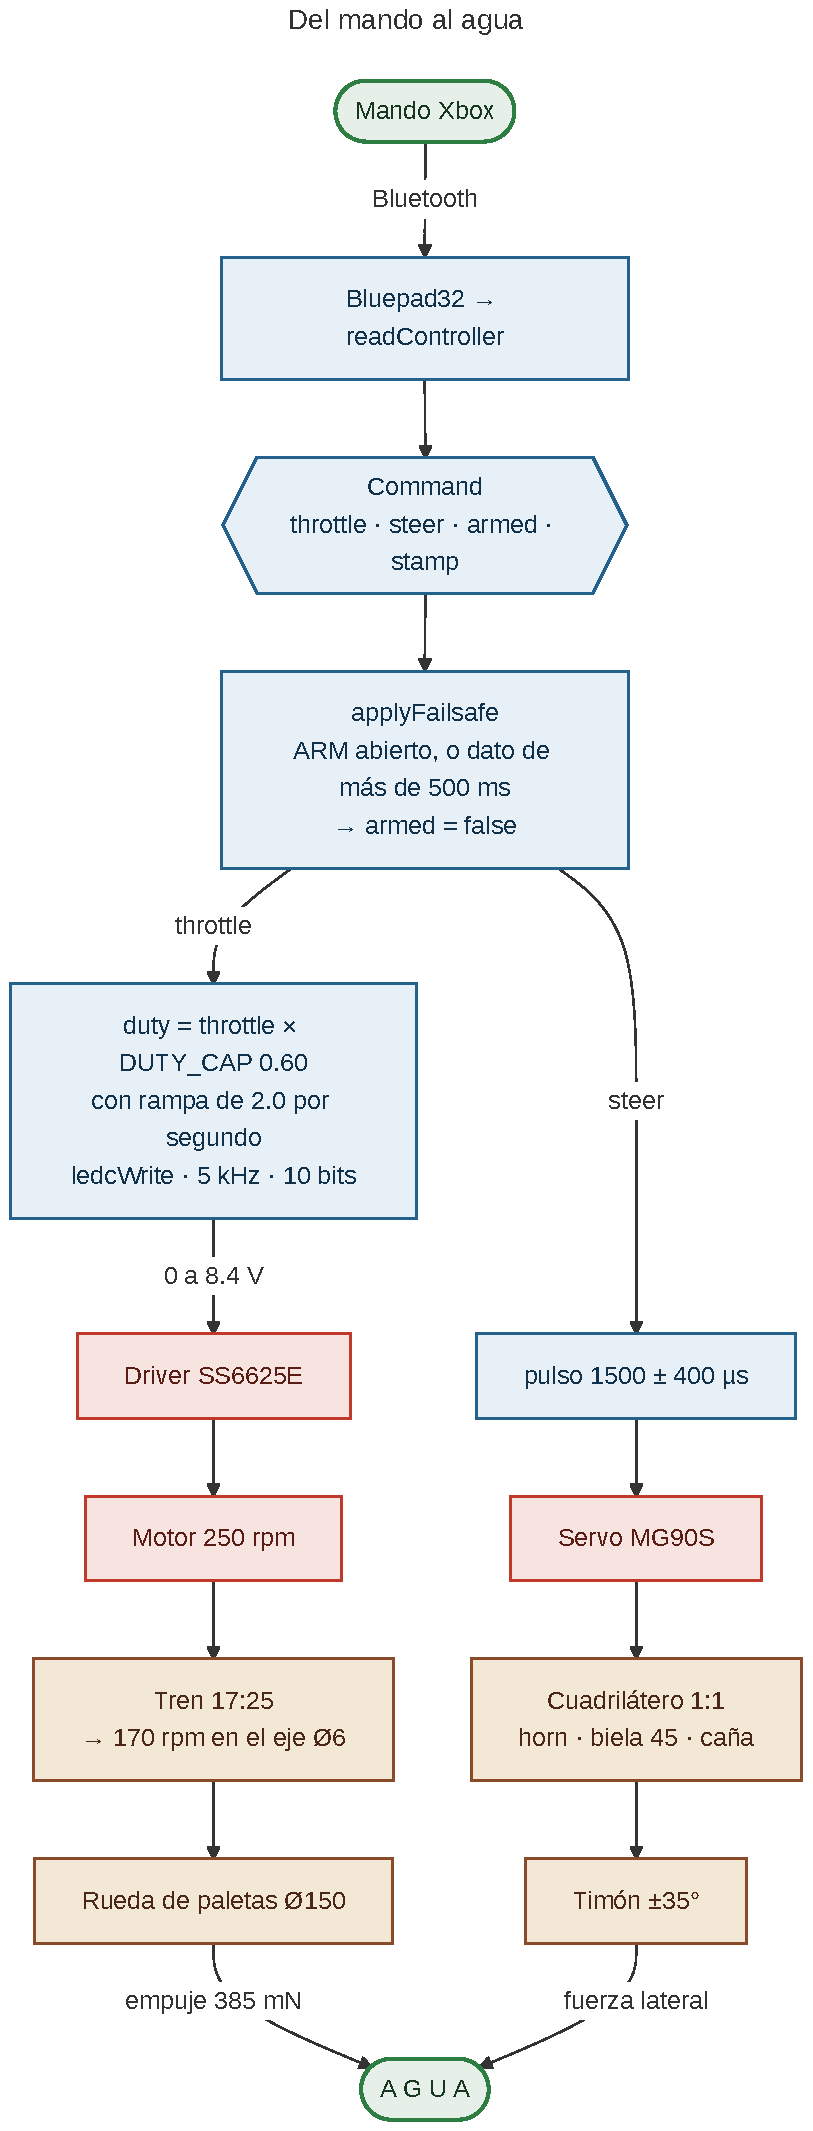
\includegraphics[height=0.78\textheight]{cadena-mando-agua.pdf}\end{center}

\clearpage
\subsection*{Lo que se ve aquí y no leyendo el código}
\begin{itemize}[leftmargin=*,itemsep=3pt]
\item \textbf{Una sola estructura \texttt{Command} alimenta las dos ramas.} Propulsión y
gobierno no son dos programas: son dos consumidores del mismo dato.
\item \textbf{El failsafe está antes de la bifurcación}, así que apaga las dos cosas a la
vez. No hay forma de quedarse con timón pero sin motor, ni al revés.
\item \textbf{Cada flecha de la mitad de abajo es una pieza física} que hay que cortar,
imprimir o pegar. La cadena mecánica es más larga que la de software.
\item \textbf{Dónde se pierde y se gana.} El tren 17:25 baja de 250 a 170 rpm y a cambio
multiplica el par por 1.47. El cuadrilátero del timón, en cambio, es \textbf{1:1 a
propósito}: brazos iguales, para que calibrar el servo sea un número por lado y no una tabla.
\end{itemize}

\section*{Cómo usarlos en clase}
\begin{enumerate}[leftmargin=*,itemsep=3pt]
\item \textbf{Antes de escribir código:} el diagrama 2 \emph{tapando la mitad de abajo}.
«¿Qué tiene que producir el firmware?» $\rightarrow$ un \texttt{Command}. Eso es todo.
\item \textbf{En Phase 5:} el diagrama 1, pero que dibujen ellos las transiciones antes de
verlo. Casi siempre se les olvida que el failsafe tiene \emph{dos} gatillos, no uno.
\item \textbf{Al final:} el diagrama 2 entero, para que vean que el \texttt{throttle} que
escribieron acaba siendo empuje en el agua a través de once cosas.
\end{enumerate}

\end{document}
